In gravity work, more than in any other branch of geophysics, large and
(in principle) calculable effects are produced by sources which are not of
direct geological interest. These effects are removed by reductions involving
sequential calculation of a number of recognized quantities.

\paragraph{Latitude correction} Because of the shape of the Earth, 
latitude has a large effect on gravity measurements, as visible in 
the following figure:

\begin{center}
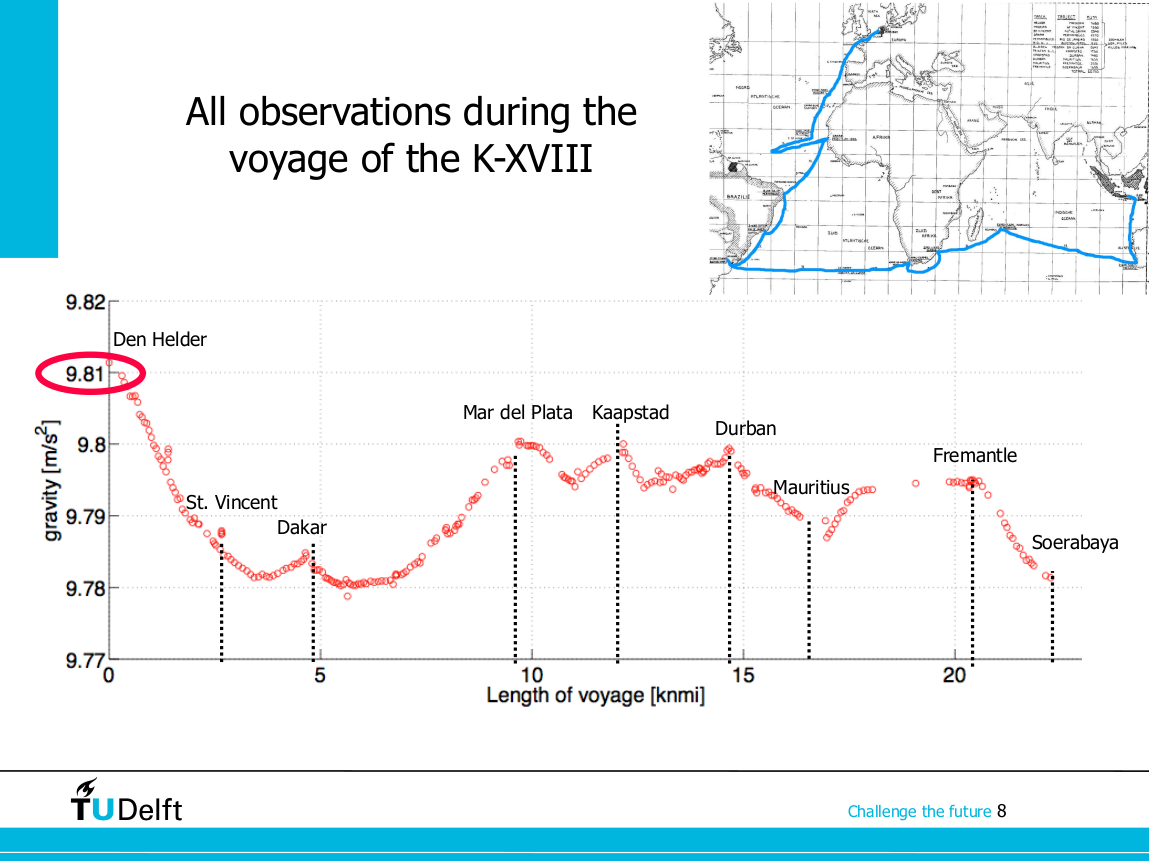
\includegraphics[width=7cm]{images/gravity/vm3}
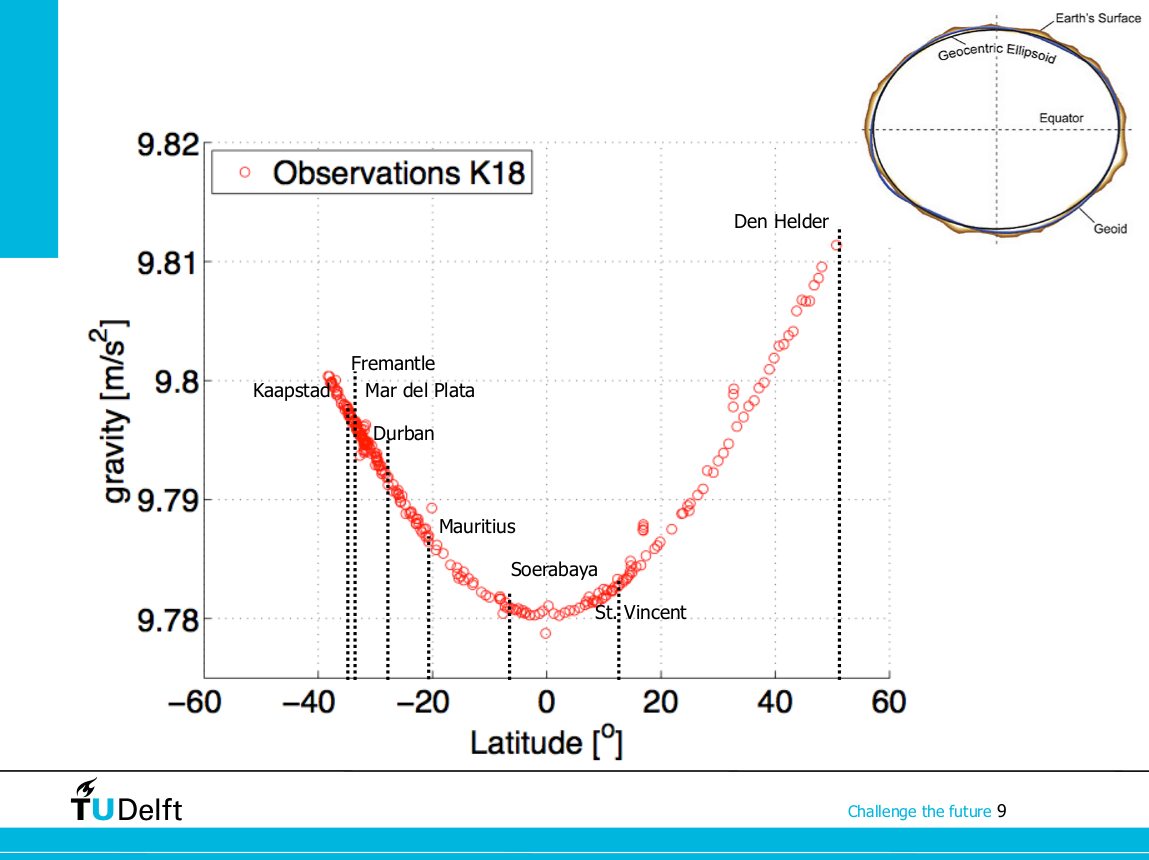
\includegraphics[width=7cm]{images/gravity/vm2}\\
{\captionfont gravity as measured by V. Meinesz onboard the K-XVIII
submarine. On the left: chronological order.\\ On the right: same 
measurements, but organised per latitude. }
\end{center}

It is obvious that we are not interested in this long wavelength pattern, but 
rather in the deviations from it. 

The formula is as follows:
\[
g_n = 978031.85 (1.0 + 0.005278895 \sin^2(lat) + 0.000023462 \sin^4(lat)) \text{(mgal)}
\]
where $lat$ is the latitude.

\paragraph{Free-air correction}

After substracting the above signal, the observed gravity will
be due in part to the height of the gravity station above the sea-level reference
surface.
An increase in height implies an increase in distance from the Earth’s
centre of mass and the effect is negative for stations above sea level ($g \propto r^{-2}$).
The free-air correction is thus positive and 
the quantity obtained after applying both the latitude and
free-air corrections is termed the free-air anomaly or free-air gravity.


\paragraph{Bouguer correction}



\paragraph{Terrain correction}


material10.pdf
